\documentclass[a4paper, 11pt]{article}
\usepackage{comment} % enables the use of multi-line comments (\ifx \fi) 
\usepackage{fullpage} % changes the margin
\usepackage[a4paper, total={7in, 10in}]{geometry}
\usepackage{amsmath,mathtools}
\usepackage{amssymb,amsthm}  % assumes amsmath package installed
\usepackage{float}
\usepackage{graphicx}
\usepackage{xcolor}
\usepackage{mdframed}
\usepackage[shortlabels]{enumitem}
\usepackage{varwidth}
\usepackage{indentfirst}
\usepackage{hyperref}
\hypersetup{
	colorlinks=true,
	linkcolor=blue,
	filecolor=magenta,      
	urlcolor=blue!70!red,
	pdftitle={Assignment 2 - Part 1},
}
\usepackage[most,many,breakable]{tcolorbox}

\definecolor{mygreen}{RGB}{56, 140, 70}
\definecolor{mytheorembg}{HTML}{F2F2F9}
\definecolor{mytheoremfr}{HTML}{00007B}

\tcbuselibrary{theorems,skins,hooks}
\newtcbtheorem{problem}{Problem}
{%
	enhanced,
	breakable,
	colback = mytheorembg,
	frame hidden,
	boxrule = 0sp,
	borderline west = {2pt}{0pt}{mytheoremfr},
	sharp corners,
	detach title,
	before upper = \tcbtitle\par\smallskip,
	coltitle = mytheoremfr,
	fonttitle = \bfseries\sffamily,
	description font = \mdseries,
	separator sign none,
	segmentation style={solid, mytheoremfr},
}
{p}

\newtcbtheorem[number within=section]{definition}{Definition}{enhanced,
	before skip=2mm,after skip=2mm, colback=red!5,colframe=red!80!black,boxrule=0.5mm,
	attach boxed title to top left={xshift=1cm,yshift*=1mm-\tcboxedtitleheight}, varwidth boxed title*=-3cm,
	boxed title style={frame code={
					\path[fill=tcbcolback]
					([yshift=-1mm,xshift=-1mm]frame.north west)
					arc[start angle=0,end angle=180,radius=1mm]
					([yshift=-1mm,xshift=1mm]frame.north east)
					arc[start angle=180,end angle=0,radius=1mm];
					\path[left color=tcbcolback!60!black,right color=tcbcolback!60!black,
						middle color=tcbcolback!80!black]
					([xshift=-2mm]frame.north west) -- ([xshift=2mm]frame.north east)
					[rounded corners=1mm]-- ([xshift=1mm,yshift=-1mm]frame.north east)
					-- (frame.south east) -- (frame.south west)
					-- ([xshift=-1mm,yshift=-1mm]frame.north west)
					[sharp corners]-- cycle;
				},interior engine=empty,
		},
	fonttitle=\bfseries,
  colbacktitle=red!75!black,
	title={#2},#1}{def}

\tcbuselibrary{theorems,skins,hooks}
\newtcbtheorem[number within=section]{note}{Note}
{%
        enhanced
        ,breakable
        ,colback = mygreen!10
        ,frame hidden
        ,boxrule = 0sp
        ,borderline west = {2pt}{0pt}{mygreen}
        ,sharp corners
        ,detach title
        ,before upper = \tcbtitle\par\smallskip
        ,coltitle = mygreen!85!black
        ,fonttitle = \bfseries\sffamily
        ,description font = \mdseries
        ,separator sign none
        ,segmentation style={solid, mygreen!85!black}
}
{th}

\newcommand{\prob}[2]{\begin{problem}{#1}{}#2\end{problem}}
\newcommand{\dfn}[2]{\begin{definition}{#1}{}#2\end{definition}}
\newcommand{\nt}[2]{\begin{note}{#1}{}#2\end{note}}


\setlength{\parindent}{0pt}

\begin{document}


\textsf{\noindent \large\textbf{Geet Sethi} \hfill \textbf{Assignment - 2 | Part - 1} \\
    \normalsize Course: Attacking LLMs Using Projected Gradient Descent \hfill Date: Jun 09, 2024}

\section{Theory}

\subsection{Lagrange's Duality}
The \emph{Lagrange's multiplier} along with \emph{KKT} conditions can be used to find the \emph{argmin}. It results in the following:
\dfn{Lagrange's Duality}{
  If $\Omega: g(x) \le c$ is a convex domain and we want to find $z = \underset{x \in \Omega}{\textrm{argmin}} \ f(x)$, then the following conditions must hold for optimality:
    \begin{itemize}
      \item If $x \in \Omega$, then $z = x$.
      \item If $x \notin \Omega$, then {
    \begin{itemize}
      \item $g(x) = c$
      \item $\nabla f(x) = \lambda \nabla g(x)$
    \end{itemize}
    Solving these two equations simultaneously will yield the result!
        }
    \end{itemize}
}

\subsection{Overview of the Projection Step}

\begin{figure}[h]
  \begin{minipage}[c]{7cm}
    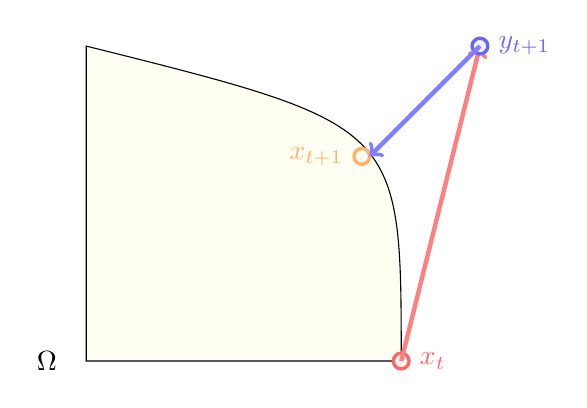
\begin{tikzpicture}
      \draw[fill=yellow!5] (-2, -2) -- (2,-2) .. controls (2,1) .. (-2,2) -- cycle node[xshift=-5mm]{$\Omega$};

      \filldraw[color=red!60!white, fill=red!5, very thick](2,-2) circle (0.1) node[anchor=west,xshift=1mm]{$x_t$};
      \draw[->,ultra thick,draw=red!50!white] (2,-2) -- (3,2);

      \filldraw[color=blue!60!white, fill=blue!5, very thick](3,2) circle (0.1) node[anchor=west,xshift=1mm]{$y_{t+1}$};
      \filldraw[color=orange!60!white, fill=orange!5, very thick](1.5,0.6) circle (0.1) node[anchor=east,xshift=-1mm]{$x_{t+1}$};
      \draw[->,ultra thick,draw=blue!50!white] (3,2) -- (1.6,0.6);
    \end{tikzpicture}
    \caption{Projection Step}
  \end{minipage}
  \begin{minipage}[c]{\textwidth-7cm}
    \begin{align*}
      y_{t+1} = x_t - \gamma \nabla f(x_t) \\
      x_{t+1} = \textrm{proj}_{\Omega} \ (y_{t+1})
    \end{align*}
    After carrying out the usual gradient descent, we apply the projection operator on the result($y_{t+1}$) to make sure that the final result ($x_{t+1}$) is contained inside the domain ($\Omega$)
   \end{minipage}
\end{figure}

\subsection{The Projection Operator}
\label{projection-operator}
\dfn{Projection Operator}{The projection operator projects the given vector ($x$) onto the domain ($\Omega$) which is a convex set. It is mathematically defined as:
\[ 
  \textrm{proj}_{\Omega}(x) = \underset{u \in \Omega}{\textrm{argmin}} \  \frac{1}{2} \lVert u - x \rVert ^2
\]
}

\newpage

\section{Problems}

%%%%%%%%%%%%%%%%%%%%%%%%%%%%%%%%%%%%%%%%%%
%               Problem 1                %
%%%%%%%%%%%%%%%%%%%%%%%%%%%%%%%%%%%%%%%%%%

\prob{}{
  Compute the projection step
  \[
    P_{\mathbb{C}}(z) = \underset{x \in \mathbb{C}}{\mathrm{argmin}} \ \frac{1}{2\gamma} \lVert x - z \rVert ^2
  \]
  where $\mathbb{C} = \{x \in \ \mathbb{R} \ | \ a^Tx \le c \}$ for some fixed $a \in \mathbb{R}^n$ and $c \in \mathbb{R}$.
}

%Solution
\setlength{\parindent}{0cm}\textbf{\textit{Solution: }}\setlength{\parindent}{1cm}
Let $\Omega = \{ x \in \mathbb{R} \ | \ a^Tx = c \}$ be the domain onto which we want to project $z$. (This $\Omega$ is the hyperplane with $n-1$ dimensions where $a^T \in \mathbb{R}^n$) \\
Therefore, taking all possible orientation (i.e. leaving one dimension at a time), we can construct a matrix $A$ with $n$ columns and $n-1$ rows. \\
$\Longrightarrow$ Our domain: $\Omega: Ax = c$ \\
\\
We know that:
\[
  \textrm{proj}_{\mathbb{C}}(z) = \underset{x \in \mathbb{C}}{\textrm{argmin}} \frac{1}{2 \gamma} \lVert x - z \rVert ^2
\]

\noindent Let $f(x, z) = \frac{1}{2} \lVert z - x \rVert ^2$ and $g(x) = Ax - c$. \\
Therefore from Lagrange's duality, we have the following conditions:
\begin{align}
  g(x) = 0 & \Rightarrow Ax - c = 0 \\
  \nonumber \nabla f(x) = \lambda \nabla g(x) & \Rightarrow \frac{1}{\gamma} \ (z - x) + \lambda \nabla g(x) = 0 & (\textrm{since } \nabla f(x) = \frac{1}{\gamma} \ (x - z)) \\
  \nonumber & \Rightarrow (z - x) + \lambda \gamma \ \nabla g(x) = 0 \\
  \nonumber & \Rightarrow (z - x) + \beta \ \nabla g(x) = 0  & (\textrm{let } \lambda \gamma = \beta) \\
            & \Rightarrow (z - x) + \beta \ A^T = 0 & (\textrm{since } \nabla g(x) = A^T)
\end{align}

Solving further, we get:
\begin{align*}
  & z - x + \beta A^T = 0 \\
  & \Rightarrow x = z + \beta A^T \\
  & \Rightarrow Ax = Az + \beta AA^T & (\textrm{pre-multiplying by } A) \\
  & \Rightarrow c = Az + \beta AA^T & (\textrm{since } g(x) = Ax - b = 0) \\
  & \Rightarrow \beta AA^T = Az - c \\
  & \Rightarrow \beta = (AA^T)^{-1} (Az - c) \\
  & \Rightarrow x = z + (AA^T)^{-1} (Az - c) A^T \\
\end{align*}

Therefore, the answer is:
$\boxed{x = z + (AA^T)^{-1} (Az - c) A^T}$

\nt{Similarity to Linear Algebra}{
  If you look closely, this result is very similar to the result derived in \emph{Linear Algebra} courses for finding the projection of a vector onto a hyperplane where we find the projection matrix!
}

\end{document}
